For the proposed approach the following parameters are significant (these
parameters, as mentioned earlier, define execution strategy): job size,
requested job walltime, job launching scheme (e.g., number of parallel job
launching streams, launching interval for consecutive jobs, etc.). Speaking
of a static strategy we mean that parameters mentioned above stay constant
during the total assessed period of time. In the current implementation of
the approach, launching scheme is defined by user, and we assess job size
and walltime that better fit for the given scheme.

Static strategy is already an improvement, but has its own limitations,
which are characterized by slow reaction on the following changes:
\begin{itemize}
    \item workload changes;
    \item resources availability (changes status from online to offline and
    backward), where time scale over availability of resources is constant.
\end{itemize}

Of course, if it would be possible to predict workload changes, then the
strategy for such expected workload changes would be adapted dynamically,
thus move from static to dynamic strategy. But it would require a prediction
with high accuracy, which is not presented in this field.

As for resources availability changes, we believe that for large and stable
supercomputers (e.g., the Titan supercomputer), commissioning or
decommissioning significant amounts of computing resources is quite rare
that can be ignored for one or two year time period.

One more restriction for static strategy implementation is a large research
time interval, which equals to large number of launched jobs and large
amount of used allocated computing time, by our estimate, namely hundreds of
thousands of core-hours and more. This is necessary to smooth local spikes
of key parameters on large time interval.

The designed approach, which is applied for supercomputers (follows job
processing scheme presented in
Figure~\ref{fig-job-processing-general-scheme}), consists of the following
steps:
\begin{itemize}
    \item Choose job launching scheme (e.g., number of parallel job
    launching streams, launching interval for consecutive jobs, etc.), time
    interval during which the specified strategy will be used, and the total
    utilization of computing resources that can be achieved.
    \item Go through all possible combinations of job size and requested
    walltime, determining probability of achieving the specified disposal in
    a given time for the chosen job launching scheme for each combination.
    \item (Optional) Repeat previous two steps for other launching schemes.
    \item Choose as the outperforming static strategy three parameters (job
    launching scheme, requested number of nodes, requested walltime), which
    gives the highest probability.
\end{itemize}

\begin{figure}
    \centering
    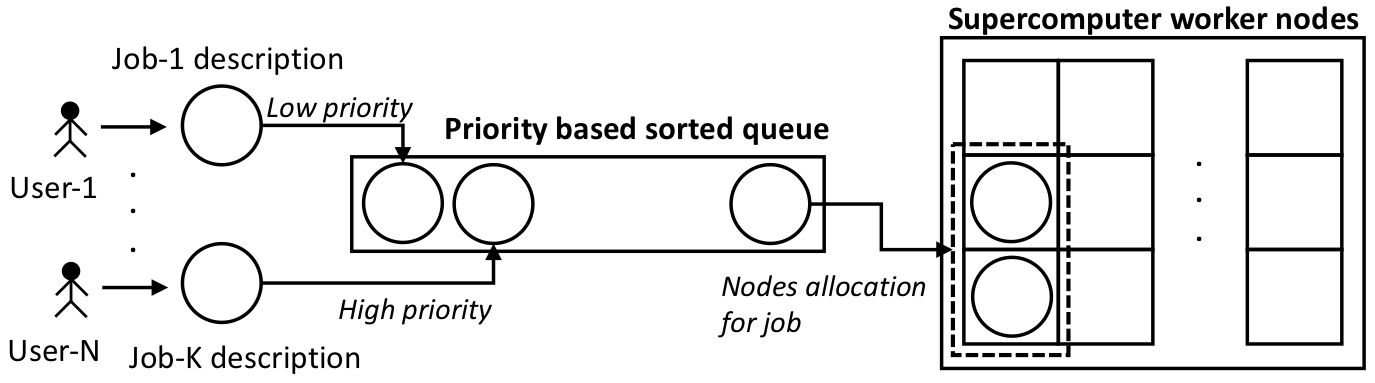
\includegraphics[width=0.45\textwidth]{pics/job-processing-general-scheme.png}
    \caption{General scheme of jobs processing at supercomputers}
    \label{fig-job-processing-general-scheme} 
\end{figure}

It is almost impossible to check through all possible combinations of job
size and requested walltime, since job size can vary from 1 core in 1 node
to the maximum allowable value (e.g., it is more than 18 thousands nodes in
the Titan supercomputer, more details are in
Section~\ref{sec-experiments-1-1}), while walltime can vary from several
minutes to several days. Therefore, we propose to group each parameter's
range into small categories, where jobs from each category can be assumed having
similar basic characteristics, such as, for example, utilization per a
single job.

In order to determine a probability of achieving a certain utilization in a
defined time interval for a specified pair $\{num\_nodes, walltime\}$, we
have developed a quantitative model. The model assists in calculation of
probability of achieving defined utilization during the defined time by jobs
of certain size with corresponding walltime (waiting time for a job in the
queue is estimated by other parameters). The model allows to set job's size,
walltime and queue waiting time as random variables with a given expectation
and variance.

To determine parameters of a random variable that specifies queue waiting
time for a job of a certain size with corresponding walltime, one can use:
\begin{itemize}
    \item recorded (historical) data;
    \item simulated (synthetic) data.
\end{itemize}

By evaluating recorded (historical) data, it is possible to filter out jobs
with similar characteristics and estimate for them queue waiting time. The
disadvantage of using only recorded (historical) data is that we cannot take
into account changes in system's workload from new jobs, that we will launch
on it. To take into account such changes, as well as to verify calculations
of the quantitative model, it is possible to use simulated (synthetic) data
from a simulator of the supercomputer load. This modeling tool was developed in
order to meet the analysis requirements.

Figure~\ref{fig-analysis-workflow} illustrates the scheme of the designed
approach, with the following workflow: i) a user sets the strategy launching
schemes; ii) similar jobs are selected from the log for the given schemes;
iii) for selected jobs, the main characteristics are defined: job size, queue
waiting time, walltime; iv) if necessary, these characteristics are refined
using the simulator; v) the parameter space is divided into categories and for
each category we calculate probability of achieving the specified utilization
using the quantitative model; vi) if necessary, utilization calculated for the
quantitative model is verified using the simulator.

\begin{figure}
    \centering
    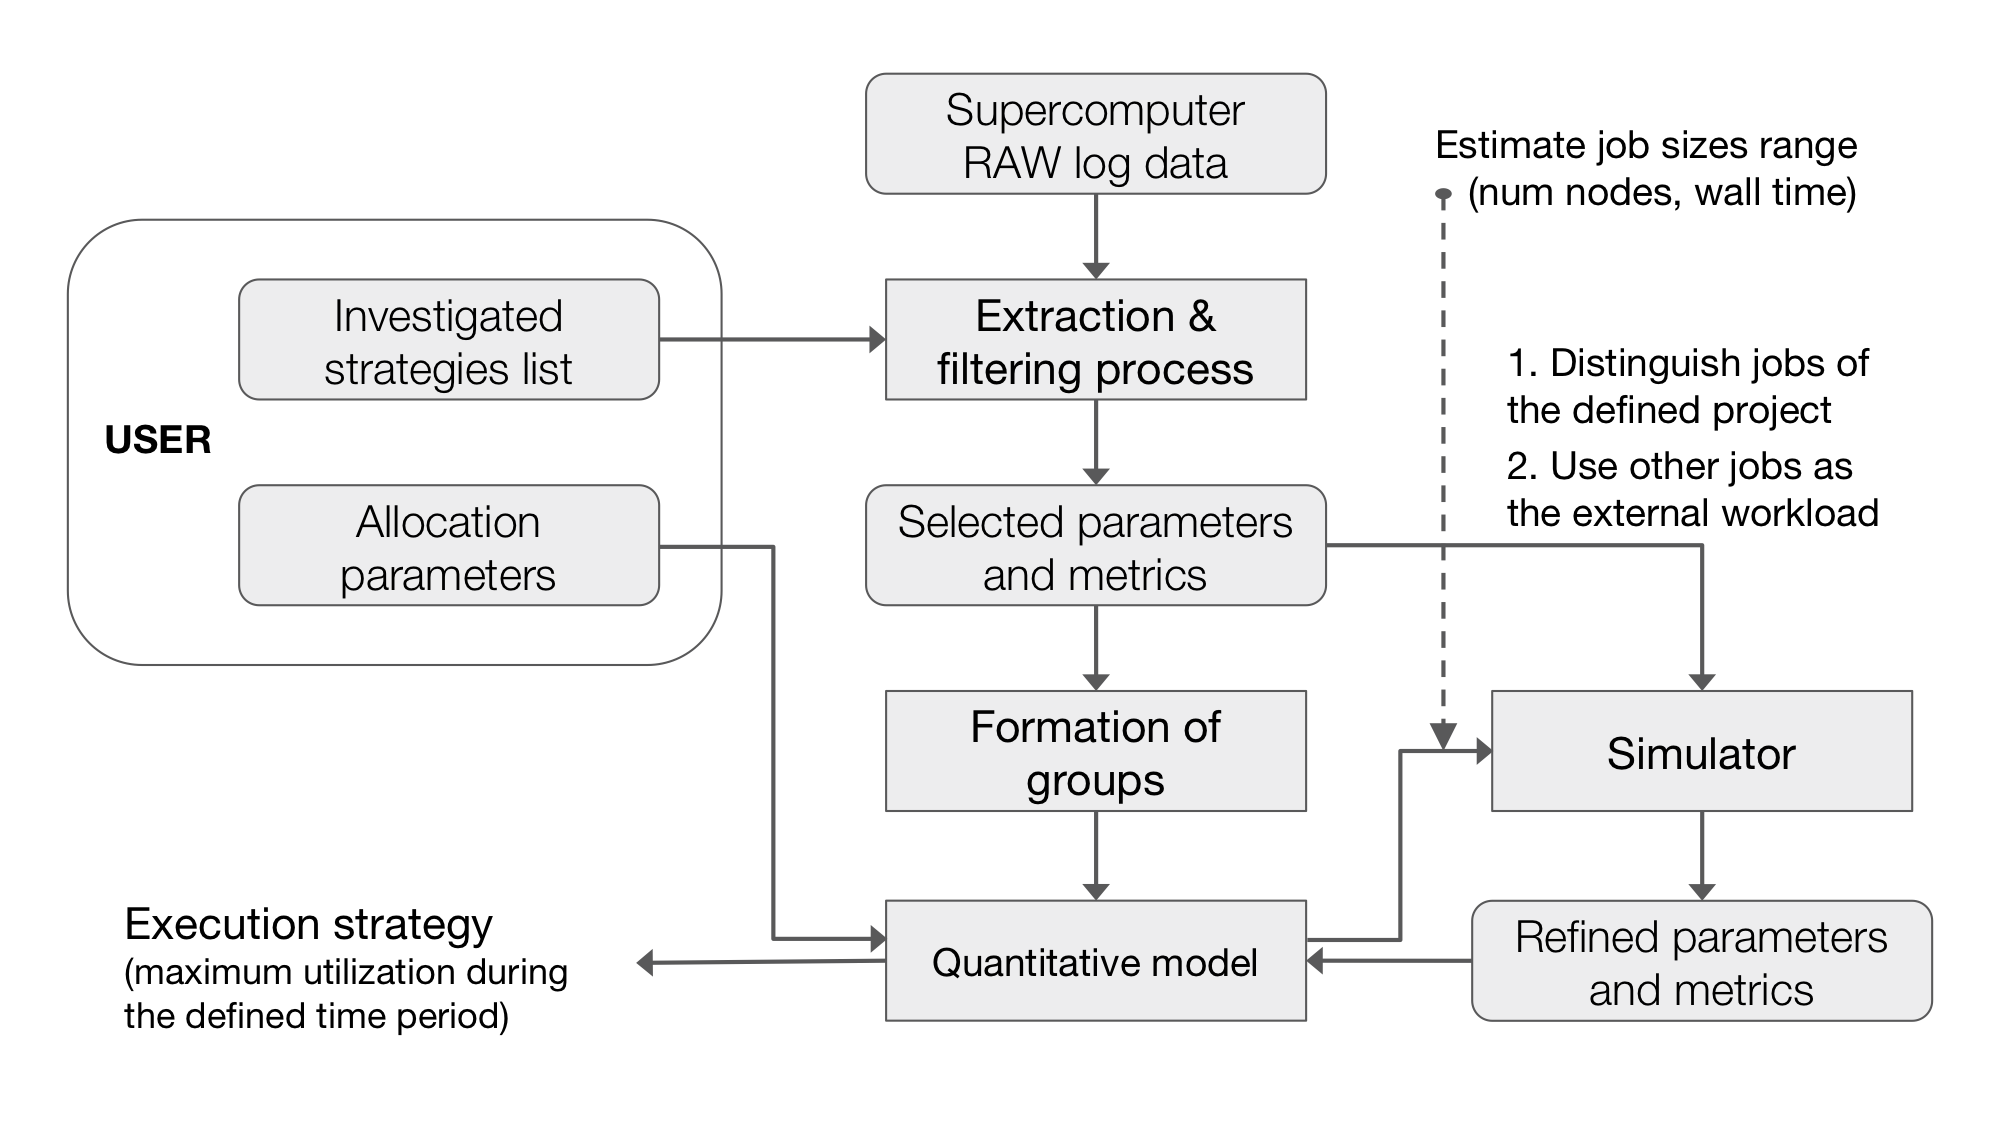
\includegraphics[width=0.48\textwidth]{pics/analysis-workflow.png}
    \caption{Workflow of the analysis process}
    \label{fig-analysis-workflow} 
\end{figure}
